%%%%%%%%%%%%%%%%%%%%%%%%%%%%%%%%%%%%%%%%%%%%%%%%%%%%%%%%%%%%%%%%%%%%%%
%%%%%%%%%%  PLANTILLA DE ARTÍCULO DE LA REVISTA TEMAT  %%%%%%%%%%%%%%%
%%%%%%%%%%%%%%%%%%%%%%%%%%%%%%%%%%%%%%%%%%%%%%%%%%%%%%%%%%%%%%%%%%%%%%

% Este archivo puede servir como plantilla a los interesados en presentar artículos a TEMat.
% Hemos intentando dejar claro el uso de los distintos comandos habituales en su uso, así como ejemplos de los más importantes.
% En caso de encontrar errores o tener problemas con las plantillas, por favor, contactad con publicaciones@anemat.com.
\documentclass[%
extracommands,% añade comandos extra, como \diff para el operador diferencial.
]{revistaanem}
%% Si estáis enviando el artículo a revisión, cargad la clase de la siguiente manera:
% \documentclass[anon]{revistaanem}

%% Carga aquí los paquetes extra que quieras, intentando que no se salgan de las recomendaciones...
%% Por ejemplo,
\usepackage{algpseudocode}

%%%%%%%%%%%%% PARA USUARIOS DE PSTRICKS Y TIKZ %%%%%%%%%%%%%%%%%
%% Os recomendamos que uséis TikZ, mejor que PSTricks.
%% En cualquier caso, os pedimos que leáis la sección <<Detalles avanzados>> dentro de <<Figuras, dibujos y diagramas>>.
%% de `PlantillaTEMat.tex'.
%%%%%%%%%%%%% Fin para usuarios de PSTricks y TikZ


%% Fin del espacio para cargar paquetes.
% Ahora ya empieza el documento en sí.
% Sí, el título y los autores van después del \begin{document}
\begin{document}
% \titulo[Título corto, opcional]{Título del artículo; escribe el corto si este llega más allá de los 3/4 del ancho de página en las cabeceras}
\titulo[Plantilla para artículos para \nombrerevista]{Plantilla para artículos para \nombrerevista{}, con teoremas que son mentira y explicaciones básicas para usar \LaTeX{} para hacer artículos}

% \autor[email_opcional]{Nombre}{Apellido/s}{Afiliación}
\autor[publicaciones@anemat.com]{Comisión de}{Publicaciones}{Asociación Nacional de Estudiantes de Matemáticas (ANEM)}
\autor{Comité editorial de}{\nombrerevista}{Asociación Nacional de Estudiantes de Matemáticas (ANEM)}
%% Estos nombres son inventados. En nombres de verdad, las partículas del apellido van con el apellido, por supuesto.
%% Se pueden añadir tantos autores como sea necesario.

\msc{00-01}
\keywords{ANEM, plantilla, instrucciones, artículos, revista, criterios de estilo}
\agradecimientos{Queremos agradecer a la ANEM el impulso a esta revista y el apoyo a jóvenes estudiantes de matemáticas. Agradecemos también a los miembros del comité editorial su labor y dedicación.
Finalmente, agradecemos a todos los autores que quieran participar en este proyecto su interés, tiempo y trabajo.

En este apartado es habitual incluir también las ayudas económicas y becas disfrutadas durante el transcurso del proyecto.}

\nuevabibliografia{plantilla.bib}
%\nuevabibliografia{plantilla2.bib}
% El resumen debe ser lo último en aparecer antes de empezar con el contenido del artículo.
\begin{resumen}
Este archivo sirve como plantilla para artículos que se quieran presentar a la revista \nombrerevista{} de la ANEM.
Presentamos de manera simple cómo se debe usar el formato de la revista, así como las instrucciones habituales y todo lo relacionado con la redacción de artículos en \LaTeX.
Se puede utilizar la propia plantilla como base para trabajar.
También discutimos los paquetes necesarios, de los cuales la mayoría se cargan automáticamente, y algunos paquetes prohibidos.
Se dan varios ejemplos de uso de la mayor parte de los elementos presentados.

Para asegurar un estilo uniforme en todos los artículos de la revista, el uso de la plantilla es obligatorio, y está totalmente prohibido cambiar los ajustes de espaciado y estructura.
\end{resumen}

\section{Introducción}

Esta es la plantilla de artículos para la revista \nombrerevista{}.
En ella recogemos todas las instrucciones básicas sobre cómo crear artículos en \LaTeX{} de acuerdo a los criterios editoriales de \nombrerevista{}.
Hay varios documentos que forman parte de la plantilla.
Los más importantes son el documento \verb+revistaanem.cls+, que forma una clase que incluye todo el formato de la revista y \textbf{NO} se debe modificar; el documento \verb+PlantillaTEMat.tex+, que sirve para crear artículos, y el documento \verb+plantilla.bib+, que sirve para crear bibliografías que después se importan al artículo.
Además, están los archivos \verb+latexmkrc+ (necesario para los que utilicen \verb+latexmk+), y \verb+triangulo.tex+ y \verb+triangulo-ps.tex+ (que proporcionan ejemplos de figuras en \verb+tikz+ y en \verb+pstrics+), así como los diagramas \verb+triangulo-precompilado.pdf+ y \verb+triangulo-ps-precompilado.pdf+ como muestra para la inclusión de figuras.
Finalmente, el documento \verb+PlantillaTEMat.pdf+ permite ver el resultado después de compilar.
Si no puedes compilar la plantilla, eso quiere decir que faltan paquetes en tu ordenador, y se deben instalar.
Si el resultado de la compilación es distinto del ofrecido en el pdf, también hay algún problema.
Se puede compilar con \verb+pdflatex+, \verb+lualatex+ o \verb+xelatex+ (preferimos uno de los dos primeros, y en principio nosotros compilaremos con el segundo).
No damos soporte a compilaciones de  que no sean en modo pdf (\verb|latex+dvips+ps2pdf| u otras).

Esta plantilla (especialmente el documento \verb+revistaanem.cls+) podría ser revisada y modificada a lo largo del tiempo.
Recomendamos a los autores que descarguen la versión más reciente de la clase para trabajar.
En caso de encontrar un error o tener algún problema, contactad con los editores de \nombrerevista{} a través del correo \email{publicaciones@anemat.com}.

\section{Portada del artículo}

Cada artículo tendrá su propia portada (para que se puedan descargar por separado y quede recogida toda la información del artículo en dicha portada), parecida a la de esta plantilla.
En esta página deberá aparecer toda la información del autor o los autores y del artículo en cuestión.
Nótese que toda la información se debe introducir después del \verb+\begin{document}+.

Se debe poner el título del artículo con el comando \verb+\titulo{}+.
Si se trata de un título largo (tanto que no cabe en la cabecera de las páginas de la revista), se deberá proporcionar también un título corto.
Para ello, se deben rellenar los dos campos como sigue: \verb+\titulo[Título corto, opcional]{Título del artículo}+.
Se puede ver un ejemplo de esto y de todo lo posterior en el archivo \verb+PlantillaTEMat.tex+ de esta plantilla.

Es necesario incluir el nombre y los apellidos del autor, así como su afiliación (en qué universidad (u otro lugar) estudia o trabaja).
También existe la posibilidad de incluir un correo electrónico, para si alguien quiere contactar al autor para preguntar más sobre el tema, pero poner esto es opcional.
Para introducir estos datos, se debe utilizar el comando \verb+\autor+ rellenando los cuatro campos como sigue: \verb+\autor[email_opcional]{Nombre}{Apellido/s}{Afiliación}+.
En caso de haber más de un autor, se deberán añadir todos ellos de la misma manera, usando la instrucción \verb+\autor+ para cada uno de ellos.
En caso de haber varios autores, el orden de los mismos se puede decidir de muchas maneras.
En el mundo de las matemáticas, la práctica más habitual es poner a los autores por orden alfabético de apellido, sin darle más énfasis a uno que a los otros, y nosotros aconsejamos esta práctica; sin embargo, mantendremos el orden en que estén en el envío.

Deberá haber una lista con las palabras clave del artículo, que se debe definir con \verb+\keywords{}+.
También se debe incluir la clasificación del tema del artículo según la MSC2010 (2010 Mathematics Subject Classification) usando \verb+\msc{}+.
Para los que no conozcan esto, se debe buscar en la página \url{http://www.ams.org/msc/msc2010.html} el código (o códigos) que mejor se correspondan con la temática del artículo que se presenta.
De ser posible, se debe poner uno solo; en caso de haber varios temas relacionados, recomendamos que no se pongan más de cinco códigos.

Debajo de esta información aparecen la fecha de recepción y de aceptación del artículo presentado.
Las que hay en la plantilla están a modo de ejemplo; estos campos los rellenarán los editores de la revista para cada artículo.

En la misma página aparecerán los agradecimientos (en caso de haberlos), así como las fuentes de financiación (en caso de haberlas).
Para introducirlas, se utiliza \verb+\agradecimientos{}+.

Finalmente, se debe proporcionar un resumen (o \textit{abstract}) del artículo que se envía.
Para ello, se define un entorno de resumen delimitado por \verb+\begin{resumen}+ y \verb+\end{resumen}+ (o \verb+abstract+).
El resumen debe aportar información suficiente como para saber de qué trata el artículo y cuáles son las aportaciones principales, pero debe ser lo suficientemente corto como para que no se salga de la portada ninguno de los campos que deben estar en ella.
El resumen se debe introducir después del resto de campos de la portada.

Para anonimizar el documento para la revisión, basta con cargar la clase \verb+revistaanem+ con la opción \verb+anonimo+ (aunque también \verb+anon+, \verb+anonymous+, \verb+revision+ o \verb+review+).
Sería así, \verb+\documentclass[anon]{revistaanem}+

Insistimos: hay ejemplos de todo en \verb+PlantillaTEMat.tex+.



\section{Creando secciones...}

Todo artículo debe seguir una estructura que convierta su lectura en algo agradable y permita seguir los argumentos con mayor facilidad.
Habitualmente, esta estructura se ve reforzada utilizando secciones y subsecciones.
Para crear una sección basta con usar el comando \verb+\section{nombre}+.
Para crear subsecciones, se debe usar \verb+\subsection{nombre}+.
Existe la posibilidad de llegar hasta las subsubsecciones, pero recomendamos encarecidamente que no se haga esto.

\subsection{...y subsecciones...}

Obviamente, en cada sección se puede introducir tanto texto como queráis.

\subsection{...y más subsecciones}

\section{Matemáticas}

La principal herramienta para un matemático al usar \LaTeX{} son las fórmulas matemáticas.
Todas las fórmulas aparecerán automáticamente en letra itálica, distinguiendo así el entorno de matemáticas del texto normal.
Para añadir fórmulas, basta con usar \verb+\(+ y \verb+\)+, y escribir la fórmula matemática entre estos delimitadores.
En su defecto, se pueden usar también \verb+$+ y \verb+$+.
Así, se pueden escribir pequeñas fórmulas en entorno matemático, como \(x^3+y^3=z^3\) o $e^{i\pi}=-1$.
Si se quiere poner fórmulas centradas y separadas del resto del párrafo, se deben emplear los delimitadores \verb+\[+ y \verb+\]+ (\textbf{no} puedes usar \verb+$$+ y \verb+$$+, puede estropear el formato de la revista\footnote{En realidad, no quieres usar los dobles dólares en ningún documento. ¿El motivo? A diferencia de otros entornos, no tienen bien ajustado el espaciado.}), para conseguir formas del estilo de
\[\sum_{i=1}^n\frac{1}{i}\approx\log n.\]
Sí, las fórmulas son parte del texto, de modo que van seguidas de los signos de puntuación correspondientes.
Si además se quiere que la fórmula quede numerada, se puede usar \verb+\begin{equation}+ y \verb+\end{equation}+, de modo que resulte
\begin{equation}\label{equa:ejemplo1}
\int_{1}^x\frac{1}{t} \diff t = \log x.
\end{equation}
Existen otras muchas formas más complejas de introducir ecuaciones, con entornos como \verb+align+ y otros muchos.
Recomendamos buscar información sobre estos entornos por internet.
También se debe buscar información sobre cómo introducir caracteres especiales y diferentes símbolos matemáticos.
Por ejemplo, para referirnos a los números naturales, enteros, etc. ($\mathbb{N}$, $\mathbb{Z}$, $\mathbb{Q}$...) se utiliza el comando \verb+\mathbb{}+.
Se puede encontrar información sobre estos símbolos en páginas como \url{https://www.artofproblemsolving.com/wiki/index.php/LaTeX:Symbols} o \url{http://detexify.kirelabs.org/classify.html} (que permite dibujar el símbolo que buscas).

A menudo es frecuente querer referirse a una ecuación que se ha escrito antes (para eso se utiliza la numeración de las fórmulas).
Así, para referirnos a la fórmula \eqref{equa:ejemplo1}, tenemos que escribir el comando \verb+\eqref{formula}+, donde el nombre de la fórmula se asigna con un \verb+\label+, como podéis comprobar en la ecuación anterior en el archivo \verb+PlantillaTEMat.tex+.
Alternativamente, se puede utilizar \verb+\cref{nombre}+.

\subsection{Entornos matemáticos}

Además del entorno básico para escribir matemáticas, los matemáticos siempre escriben teoremas, corolarios, demostraciones..., y para cada uno de los tipos de enunciado hay un entorno propio.
\textbf{Se deben usar estos entornos para mantener el estilo de la revista}.
Para usar cada uno de ellos se debe empezar con un \verb+\begin{nombreentorno}+ y terminar con un \verb+\end{nombreentorno}+.
Por ejemplo, podemos escribir teoremas como los que siguen.

\begin{teorema}[del punto gordo]\label{teor:ejemplo1}
Dadas tres \emph{rectas} $r$, $s$ y\/ $t$ en $\mathbb{R}^2$, existe un punto tal que las tres rectas se intersecan en él (vaya, que se cortan).
\end{teorema}

\begin{demostracion}
Basta con tomar un punto suficientemente gordo.
\end{demostracion}

\begin{teorema}\label{teor:ejemplo2}
Contrario a la creencia común,
\[\frac{0}{0}=2.\]
\end{teorema}

\begin{demostracion}[Demostración por simplificación de ceros]
Lo demostramos con la siguiente cadena de igualdades:
\[\frac{0}{0}=\frac{100-100}{100-100}=\frac{(10+10)(10-10)}{10\,(10-10)}=\frac{20}{10}=2.\qedhere\]
\end{demostracion}

\begin{nota*}
En general, vamos a intentar que teoremas de este estilo que mandéis no se publiquen. Os vigilamos.
\end{nota*}

Para añadir información al encabezado del teorema (como un nombre, autor, año...) se debe incluir entre corchetes (\verb+[]+) después del \verb+\begin{teorema}+, como en el \autoref{teor:ejemplo1}.
Además, hay un detalle importante en cuanto a las demostraciones.
El cuadradito negro aparecerá automáticamente al final de la demostración, pero no estará bien colocado si la demostración acaba con una fórmula.
En ese caso, se debe incluir la instrucción \verb+\qedhere+ al final de la última fórmula, como sucede en la demostración del \autoref{teor:ejemplo2}.

Los entornos que hemos habilitado son teorema, proposición, corolario, lema, propiedad, conjetura, hecho, criterio, axioma, definición, ejemplo, ejercicio, problema, pregunta, hipótesis, observación, convención, nota, notación, afirmación, caso, algoritmo, solución y, por supuesto, demostración.
Para crear cualquiera de ellos, pon su nombre (sin tilde) en \verb+nombreentorno+, o sus nombres habituales en inglés, o alguna de las abreviaciones más habituales (no garantizamos que tu abreviación favorita vaya a funcionar; si no funciona, escribe el nombre completo).
No, no hay más entornos.
Si crees que alguno más es absolutamente necesario, ponte en contacto con nosotros.

En general, cada vez que se empiece a trabajar en un entorno, este aparecerá numerado.
Si el autor quiere que no sea así, basta con añadir un asterisco (\verb+*+) después de \verb+nombreentorno+ (por ejemplo, \verb+teorema*+).

También es muy frecuente querer referirnos a resultados que ya hemos escrito, como el \autoref{teor:ejemplo1}. Para hacerlo, basta con usar \verb+\autoref{nombreteorema}+ o \verb+\cref{nombreteorema}+, donde al teorema se le ha dado un nombre usando \verb+\label+ (de nuevo, puedes comprobar cómo en el archivo \verb+PlantillaTEMat.tex+).
Haciendo esto, si tienes el documento en pdf, puedes pinchar en \autoref{teor:ejemplo2} para que te muestre directamente el resultado al que se refiere, cosa muy útil a la hora de leer artículos.

\subsection{Sistema Internacional}

Para escribir números grandes o magnitudes físicas, hemos cargado el paquete \verb+siunitx+.
Si queréis saber cómo se usa, solamente tenéis que echarle un vistazo a la documentación~\cite{siunitx}.
Brevemente, para escribir un número como \num{10000}, usa \verb+\num{10000}+ (y así se verá el espacio recomendado cuando hay más de cuatro cifras).
Esperamos que el \SI{100}{\percent} de los autores que usen unidades en sus artículos aprovechen su uso.
Especialmente porque, como dice \citet{bezosOM}, las unidades se escriben en letra redonda y con un espacio entre el número y la unidad.
Por ejemplo, para escribir \SI{9.8}{m.s^{-2}} se puede usar \verb+\SI{9.8}{m.s^{-2}}+ o bien \verb+\SI{9.8}{\metre\per\square\second}+.

\section{Paquetes}

Hay determinados paquetes que se cargan de manera automática al utilizar la clase \verb+revistaanem+.
Estos paquetes tienen que estar instalados para que el archivo pueda compilar y se pueda trabajar con las plantillas de la revista.
Por supuesto, no hace falta volver a cargar estos paquetes en el preámbulo de vuestro documento.
Los paquetes que utilizamos (y que no se pueden quitar) son \verb+xkeyval+, \verb+letltxmacro+, \verb+ifxetex+, \verb+ifluatex+, \verb+ifpdf+, \verb+afterpackage+, \verb+calc+, \verb+etoolbox+, \verb+amsmath+, \verb+amssymb+, \verb+amsthm+, \verb+cabin+, \verb+newtxmath+,  \verb+thmtools+, \verb+l3regex+, \verb+xparse+, \verb+mathastext+, \verb+stackengine+, \verb+scalerel+, \verb+babel+ (con las opciones \verb+british+ y \verb+spanish+), \verb+siunitx+, \verb+mleftright+, \verb+cancel+, \verb+csquotes+, \verb+graphicx+, \verb+caption+, \verb+subcaption+, \verb+biblatex+ \verb+geometry+, \verb+xcolor+, \verb+enumitem+, \verb+titlesec+, \verb+fancyhdr+, \verb+hyperref+, \verb+cleveref+ y \verb+standalone+.
Además, si usas LaTeX estándar, se cargan también \verb+fontenc+, \verb+inputenc+, \verb+erewhon+ e \verb+inconsolata+; con LuaLaTeX y XeLaTeX se carga \verb+fontspec+, y las tipografías \verb+Erewhon+ e \verb+Inconsolatazi4+.
Y para pdfLaTeX y LuaLaTeX en modo PDF, también se carga el paquete \verb+microtype+.

Por otra parte, hay otros muchos paquetes que no incluimos obligatoriamente, pero que muchos de vosotros querréis usar.
Para utilizarlos, basta con que los carguéis de la forma habitual.

\subsection{Figuras, dibujos y diagramas}\label{sec:diagramas}
En muchos artículos puede ser interesante insertar una imagen que ayude a comprender aquello que estamos explicando.
Como norma general, dibujos, diagramas e imágenes en general deberían aparecer como figuras autocontenidas.
¿Qué queremos decir con autocontenidas?
Pues que se puedan entender por sí solas, sin necesidad de tener que leer detalladamente el texto.
Para ello, es bueno que estén dentro de un entorno \verb+figure+ y tengan una etiqueta descriptiva usando el comando \verb+caption+.
Podéis ver un ejemplo de ello en la \cref{fig:triangulos}, que además tiene subfiguras.
Igual que con las secciones y demás entornos, se puede usar el comando \verb+\label+ para referirse a ellas más tarde.

\begin{figure}[h]
  \centering
  \begin{subfigure}[b]{0.31\textwidth}
    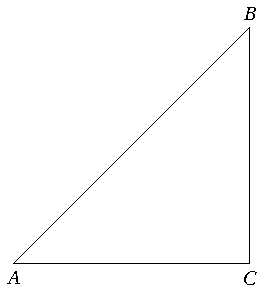
\includegraphics[width=\textwidth]{triangulo-precompilado} % el nombre del archivo SIN la extensión (mejor)
    \caption{Un triángulo hecho con TikZ.}\label{fig:triangulo-tikz}
  \end{subfigure}
  \hspace{0.1\textwidth}
  \begin{subfigure}[b]{0.31\textwidth}
    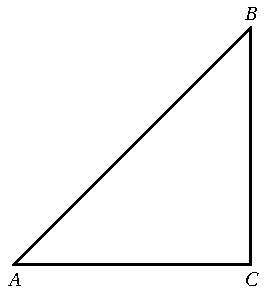
\includegraphics[width=\textwidth]{triangulo-ps-precompilado} % el nombre del archivo SIN la extensión (mejor)
    \caption{Un triángulo hecho con PSTricks.}\label{fig:triangulo-pst}
  \end{subfigure}
  \caption{Ejemplo de figura y subfiguras con TikZ y PSTricks.}\label{fig:triangulos}
\end{figure}

Si os fijáis bien en el contenido de las \cref{fig:triangulo-tikz,fig:triangulo-pst}, veréis que hemos usado el comando \verb+\includegraphics+.
Podéis encontrar más información sobre su uso en la documentación del paquete \verb+graphicx+~\cite[sec.~4]{graphics}.

\subsubsection{Información avanzada}\label{sec:diagramas:avanzado}
Hemos probado tanto \verb+tikz+ como \verb+pstricks+.
En el caso de usar TikZ, que es el que os recomendamos entre los dos, podéis cargar directamente el paquete \verb+tikz+ en el preámbulo del documento.
Sin embargo, preferimos que aprovechéis el paquete \verb+standalone+ que hemos cargado automáticamente con la clase \verb+revistaanem+, y que aprovechéis también que hemos preparado una opción \verb+standalone+ para la clase \verb+revistaanem+.

La mayor ventaja de usar \verb+standalone+ es que permite compilar las imágenes por separado (podéis probarlo con los ejemplos).
Por ejemplo, el archivo \verb+triangulo.tex+ contiene el código TikZ para dibujar la \cref{fig:triangulo-tikz}.
Para incluirlo, hemos usado el comando \verb+\imagentikz+.
Del mismo modo, \verb+triangulo-ps.tex+ tiene el código PSTricks para la \cref{fig:triangulo-pst} y se puede incluir usando \verb+\imagenpstricks+.
Estos comandos aceptan las mismas opciones que \verb+\includegraphics+, pero en este caso no debe incluirse la extensión del fichero.
Así, por ejemplo, la \cref{fig:triangulos} podríamos haberla incluido como sigue:
\begin{verbatim}
\begin{figure}[h]
  \centering
  \begin{subfigure}[b]{0.31\textwidth}
    \imagentikz[width=\textwidth]{triangulo}
    \caption{Un triángulo hecho con TikZ.}\label{fig:triangulo-tikz}
  \end{subfigure}
  \hspace{0.1\textwidth}
  \begin{subfigure}[b]{0.31\textwidth}
    \imagenpstricks[width=\textwidth]{triangulo-ps}
    \caption{Un triángulo hecho con PSTricks.}\label{fig:triangulo-pst}
  \end{subfigure}
  \caption{Ejemplo de figura y subfiguras con TikZ y PSTricks.}\label{fig:triangulos}
\end{figure}
\end{verbatim}

Es importante que al compilar un documento que use estos comandos, o cualquier otro de los que muestra el paquete \verb+standalone+ en su documentación~\cite{standalone} para incluir archivos externos, incluyáis la opción \verb+-shell-escape+ (a veces \verb+-enable-write18+ con MiK\TeX).
Os recomendamos que os leáis la \cref{sec:apuntes} para más información sobre la compilación.

Usar TikZ o PSTricks tiene resultados muy bonitos en formato vectorial.
Pero, evidentemente, se pueden incluir figuras hechas de cualquier otra forma, en formato pdf (por ejemplo), de la forma habitual, usando el comando \verb+\includegraphics+ del paquete \verb+graphicx+ que ya hemos incluido automáticamente.

\begin{nota}
Si tenéis conocimientos algo más avanzados de \LaTeX{}, estos dos comandos para incluir diagramas no son más que alias del comando \verb+\includestandalone+ con la opción \verb+mode=buildnew+.
Además, en el caso de PSTricks, incluye explícitamente la opción de compilar con \verb+xelatex+ porque ni \verb+pdflatex+ ni \verb+lualatex+ son compatibles.
\end{nota}

\subsection{Algoritmos}
Podéis usar los paquetes \verb+algpseudocode+ (sin la opción \verb+noend+) o \verb+program+, aunque tenemos preferencia por \verb+algpseudocode+ (que está dentro de \verb+algorithmicx+~\cite{algorithmicx}).
Para evitar incompatibilidades, consultadnos antes de usar cualquier otro paquete de algoritmos.

\begin{algoritmo}[escritura a ordenador]
\begin{algorithmic}[1]
\Procedure{Escritura}{}
\If{ordenador apagado}
\State encender ordenador
\If{ordenador apagado}
\If{ordenador enchufado}
\If{no hay corriente}
\State ... \Comment{El lector sabrá qué hacer}
\Else
\State ordenador roto
\EndIf
\EndIf
\Else
\State ... \Comment{Lo dejamos como ejercicio}
\EndIf
\EndIf
\EndProcedure
\end{algorithmic}
\end{algoritmo}

\subsection{Configuraciones y paquetes prohibidos}
\textbf{Bajo ningún concepto} deben usarse los paquetes o configuraciones que aquí indicamos:
\begin{itemize}
\item \verb+natbib+ o cualquier otro paquete de bibliografía.
  Ya usamos \verb+biblatex+ con \verb+biber+, así que habría incompatibilidades.
\item \verb+setspace+, \verb+savetrees+ o cualquier paquete que permita cambiar el espaciado del texto.
  Eso implica que aunque carguemos nosotros el paquete \verb+geometry+ no deberíais usar los comandos \verb+geometry+, \verb+newgeometry+ y similares.
  Por supuesto, tampoco debéis usar el comando \verb+\setlength+ para cambiar márgenes ni ninguna medida del documento, salvo cosas propias vuestras.
\item Cualquier paquete que cambie las tipografías.
\end{itemize}

\section{Uso de la bibliografía}

Una de las partes más importantes de un artículo divulgativo es una buena bibliografía que permita, por un lado, comprobar de dónde se ha obtenido la información que se ha utilizado para redactar el artículo y, por otro, obtener fuentes en las que leer más información sobre el tema.
Para crear una bibliografía adecuada \textbf{se debe utilizar el paquete \texttt{biblatex}} con el \extranj{english}{backend} \verb+biber+ (que cargamos automáticamente) creando un fichero externo \verb+.bib+ con la bibliografía completa.
Entre los archivos de la plantilla hay un fichero llamado \verb+plantilla.bib+ que debería servir como ejemplo de uso de este tipo de archivos.
En cualquier caso, casi siempre se pueden encontrar sitios de los que copiar directamente la bibliografía en formato bibtex (se pueden buscar las referencias, por ejemplo, en MathSciNet \url{http://www.ams.org/mathscinet/}) o en Google Scholar (\url{https://scholar.google.com/})).
Para incluir la bibliografía en el artículo, se debe emplear el comando \verb+\nuevabibliografia{archivobibliografia.bib}+ antes del resumen del artículo, como se puede ver en el archivo \verb+PlantillaTEMat.tex+, donde \verb+archivobibliografia.bib+ es el nombre que tenga vuestro documento (siempre debe ser un \verb+.bib+).
Para cargar la bibliografía, se debe escribir \verb+\printbibliography+ al final del documento, donde se quiera que vaya la bibliografía.

Para referirse a elementos de la bibliografía, a cada uno de estos elementos se le asigna un nombre en el archivo \verb+.bib+.
Luego basta con usar la instrucción \verb+\cite{nombrereferencia}+ para que aparezca, proporcionando además un vínculo a la bibliografía del final del artículo.

Toda la información sobre esto, y otras muchas cosas relacionadas con la bibliografía, la podéis encontrar en la documentación de \verb+biblatex+~\cite{biblatex}.
Si queréis buscar la versión más actualizada, es fácil encontrarla en su página de CTAN.\footnote{Acrónimo de \emph{Comprehensive \protect\TeX{} Archive Network}, ver \url{https://www.ctan.org/pkg/biblatex} y \url{https://www.ctan.org/}}
En esa misma web se pueden encontrar manuales de uso de casi todos los paquetes de \LaTeX.

\begin{nota}
El comando \verb+\printbibliography+ hará que aparezcan solo los elementos que se han citado a lo largo del artículo.
Si hay alguna referencia que no se ha citado pero que también debería aparecer, se debe usar el comando \verb+\nocite{nombrereferencia}+.
Para que aparezcan todas las que no se han citado, se puede usar un asterisco: \verb+\nocite{*}+.
\end{nota}

\begin{nota}
Para mejorar la calidad del texto, es recomendable no usar la salida del comando \verb+\cite+ como un sustantivo.
Como ejemplo, es mejor decir <<en la documentación de \texttt{biblatex}~\cite{biblatex} hay más información>> que <<en~\cite{biblatex} hay más información>>.

También existe el comando \verb+\citet+ para referirse a un trabajo nombrando al autor.
Es bueno cuando quieres decir cosas del tipo <<\citet{bezosOM} muestra gran cantidad de información sobre cómo se deberían escribir las matemáticas a ordenador>>. Otra opción es usar \verb+\citeauthor+ combinado con \verb+\cite+, como en <<\citeauthor{bezosOM} muestra gran gantidad de información sobre cómo se deberían escribir las matemáticas a ordenador~\cite{bezosOM}>>, aunque recomendamos usar \verb+\citet+.
\end{nota}

\section{Algunos apuntes}\label{sec:apuntes}
La compilación de documentos escritos con \LaTeX{} es un poco odisea, los que seáis usuarios habituales ya lo sabréis.
Si no se usan paquetes como \verb+minted+ o lo expuesto en la \cref{sec:diagramas:avanzado}, basta con ejecutar los comandos
\begin{verbatim}
pdflatex PlantillaTEMat
biber PlantillaTEMat
pdflatex PlantillaTEMat
pdflatex PlantillaTEMat
\end{verbatim}
desde la consola, sustituyendo el comando \verb+pdflatex+ por \verb+lualatex+ si es el caso y \verb+PlantillaTEMat+ por el nombre del archivo \TeX{} que se esté compilando.

Si se usan paquetes que tienen que hacer llamadas externas (\verb+minted+ o imágenes TikZ o PSTricks externalizadas) es necesario compilar en modo \extranj{english}{shell escape}:
\begin{verbatim}
pdflatex -shell-escape PlantillaTEMat
biber PlantillaTEMat
pdflatex -shell-escape PlantillaTEMat
pdflatex -shell-escape PlantillaTEMat
\end{verbatim}

Una forma más fácil de compilar el documento es usar la herramienta \verb+latexmk+, que viene por defecto en las últimas versiones de \TeX~Live y de MiK\TeX{}, aunque en Windows es necesario instalar alguna implementación de Perl como ActivePerl\footnote{\url{http://www.activestate.com/activeperl/downloads}} para que funcione.
Con esto, y mediante el archivo \verb+latexmkrc+ que incluimos con la plantilla, basta con hacer
\begin{verbatim}
latexmk PlantillaTEMat
\end{verbatim}
y el propio \verb+latexmk+ se encarga de llamar todas las veces que haga falta a cada una de las herramientas, y la opción \verb+-shell-escape+ ya la tiene activada.
Se puede editar el archivo \verb+latexmk+ con un editor de texto plano y cambiar \verb+lualatex+ por \verb+pdflatex+ en caso de preferirlo.

Todavía más fácil es usar Overleaf\footnote{\url{https://www.overleaf.com/}} o ShareLaTeX.\footnote{\url{https://www.sharelatex.com/}}
Basta con subir los archivos de la plantilla y \emph{voilà}, funciona.
En ambos casos os recomendamos que lo configuréis para que use LuaLaTeX, ya que es el formato con el que compilaremos nosotros.
Es cierto que podéis usar pdfLaTeX si lo preferís, la apariencia será prácticamente igual pero compilará más rápido (aunque en el caso de Overleaf hay que cambiarlo también en el archivo \verb+latexmkrc+).

Si usáis un editor con botones para compilar, buscad la información para configurarlo.
Muchas veces permiten el uso de \verb+latexmk+, así que lo mejor sería hacer que así fuera.
Si vais a compilar la plantilla de ejemplo, usáis \verb+minted+ o alguno de los comandos para incluir imágenes TikZ o PSTricks, aseguraos de que el comando de compilación tenga activado el \extranj{english}{shell escape}.

\section{Conclusiones}

En función del artículo, puede ser adecuado incluir para terminar una sección de conclusiones, preguntas abiertas sobre el tema, formas de obtener más información...
Algo que permita cerrar el artículo.

Este plantilla no puede ser, ni mucho menos, una introducción al enorme mundo de \LaTeX.
Para aprender más, recomendamos buscar información por internet, donde hay gran cantidad de fuentes~\cite{wiki:latex, stackexchange, texample}.

Si necesitáis algo o tenéis dudas sobre la revista, escribid a \email{publicaciones@anemat.com}.

\nocite{*}
\printbibliography[heading=bibintoc]

\end{document}
